\documentclass[11pt]{report}
% ===== Préambule commun aux documents Séries Chronologiques =====
\usepackage[utf8]{inputenc}
\usepackage[T1]{fontenc}
\usepackage[french]{babel}
\usepackage{lmodern}
\usepackage{amsmath,amssymb,amsthm,mathtools}
\usepackage{geometry}
\geometry{a4paper,margin=2.3cm}
\usepackage{enumitem}
\usepackage{array,booktabs,longtable}
\usepackage{xcolor}
\usepackage[most]{tcolorbox}
\usepackage{etoolbox}
\usepackage{graphicx}
\graphicspath{{figs/}}
\usepackage{caption}
\captionsetup{font=small,labelfont={bf,color=insea}}
\usepackage{fancyhdr}
\usepackage{titlesec}
\usepackage{hyperref}
\hypersetup{colorlinks=true,linkcolor=blue!55!black,urlcolor=blue!55!black,
  citecolor=blue!55!black,bookmarksopen=true}
\usepackage{bookmark}

% --- Couleurs ---
\definecolor{insea}{RGB}{0,76,128}
\definecolor{insealight}{RGB}{232,240,247}
\definecolor{vert}{RGB}{0,120,70}
\definecolor{vertlight}{RGB}{232,245,238}
\definecolor{orange}{RGB}{190,90,0}
\definecolor{orangelight}{RGB}{252,242,228}
\definecolor{gris}{RGB}{90,90,90}

% --- En-têtes / pieds ---
\pagestyle{fancy}
\fancyhf{}
\fancyhead[L]{\small\color{gris}\leftmark}
\fancyhead[R]{\small\color{gris}Séries Chronologiques}
\fancyfoot[C]{\thepage}
\renewcommand{\headrulewidth}{0.4pt}
\renewcommand{\footrulewidth}{0pt}

% --- Titres de section colorés ---
\titleformat{\section}{\Large\bfseries\color{insea}}{\thesection.}{0.6em}{}
\titleformat{\subsection}{\large\bfseries\color{insea!85!black}}{\thesubsection.}{0.6em}{}
\titleformat{\subsubsection}{\bfseries\color{gris}}{\thesubsubsection.}{0.6em}{}

% --- Théorèmes (pour le cours) ---
\theoremstyle{definition}
\newtheorem{definition}{Définition}[section]
\newtheorem{exemple}{Exemple}[section]
\newtheorem{remarque}{Remarque}[section]
\newtheorem{methode}{Méthode}[section]
\theoremstyle{plain}
\newtheorem{theoreme}{Théorème}[section]
\newtheorem{proposition}{Proposition}[section]
\newtheorem{corollaire}{Corollaire}[section]
\newtheorem{propriete}{Propriété}[section]

% --- Boîtes ---
\newtcolorbox{recette}[1][]{colback=vertlight,colframe=vert,
  fonttitle=\bfseries,title={Recette d'examen\ifblank{#1}{}{ --- #1}}}
\newtcolorbox{attention}[1][]{colback=orangelight,colframe=orange,
  fonttitle=\bfseries,title={Attention\ifblank{#1}{}{ --- #1}}}
\newtcolorbox{rappel}[1][]{colback=insealight,colframe=insea,
  fonttitle=\bfseries,title={Rappel de cours\ifblank{#1}{}{ --- #1}}}
\newtcolorbox{reponse}[1][]{colback=vertlight,colframe=vert!70!black,
  left=2mm,right=2mm,top=1mm,bottom=1mm,boxrule=0.8pt,#1}

% --- Notations Séries Chronologiques ---
\newcommand{\E}{\mathbb{E}}
\newcommand{\Var}{\operatorname{Var}}
\newcommand{\Cov}{\operatorname{Cov}}
\newcommand{\Corr}{\operatorname{Corr}}
\newcommand{\cor}{\operatorname{cor}}
\newcommand{\BB}{\operatorname{BB}}
\newcommand{\R}{\mathbb{R}}
\newcommand{\Z}{\mathbb{Z}}
\newcommand{\N}{\mathbb{N}}
\newcommand{\Xhat}{\widehat{X}}
\newcommand{\phihat}{\widehat{\phi}}
\newcommand{\rhohat}{\widehat{\rho}}
\newcommand{\gammahat}{\widehat{\gamma}}
\newcommand{\eps}{\varepsilon}
\DeclareMathOperator{\sgn}{sgn}

% Étiquette « bonne réponse » pour les QCM (utilisée dans le corrigé)
\newcommand{\bonne}[1]{\textbf{\color{vert}#1}}
\newcommand{\horsprog}{\textsuperscript{\color{orange}\,$\star$}}

\usepackage{amsfonts}

\renewcommand{\chaptermark}[1]{\markboth{\thechapter.\ #1}{}}
\titleformat{\chapter}[display]
{\normalfont\huge\bfseries\color{insea}}{\chaptertitlename\ \thechapter}{12pt}{\Huge}
\titlespacing*{\chapter}{0pt}{-20pt}{18pt}

\title{\vspace{-1.5cm}\textbf{\color{insea}Séries Chronologiques}\\[3mm]
\large Cours complet, entièrement démontré et illustré\\[1mm]
\normalsize orienté vers la résolution des exercices d'examen\\[2mm]
\normalsize\itshape d'après le cours de Fadoua BADAOUI (INSEA)}
\author{Préparation au module}
\date{\today}

\begin{document}
\maketitle
\thispagestyle{empty}

\begin{tcolorbox}[colback=insealight,colframe=insea,title={Esprit de ce cours}]
Ce cours est \textbf{recentré sur les notions effectivement évaluées} dans le recueil
d'examens : tout ce qui n'est exploité par aucune question (descriptions logicielles,
test de Fisher, tableau de Buys--Ballot détaillé, etc.) a été \textbf{retiré}. En revanche,
chaque notion utile est \textbf{entièrement démontrée}, \textbf{développée} et
\textbf{illustrée graphiquement}, avec des encadrés :
\begin{itemize}[leftmargin=*,nosep]
\item \textbf{\color{vert}Recette d'examen} : la méthode pas-à-pas, reliée aux questions (Q\,A.x\dots).
\item \textbf{\color{insea}Lecture graphique} : comment interpréter une figure.
\item \textbf{\color{orange}Attention} : pièges classiques.
\end{itemize}
\noindent\textbf{Notations.} $(X_t)_{t\in\Z}$ ; $B$ opérateur retard ($B^kX_t=X_{t-k}$) ;
$a_t\sim\BB(0,\sigma^2)$ bruit blanc ; $\gamma(k)$ autocovariance ; $\rho(k)=\gamma(k)/\gamma(0)$
autocorrélation (ACF) ; $P(k)$ autocorrélation partielle (FAP/PACF).
\end{tcolorbox}

\newtcolorbox{lecture}[1][]{colback=insealight,colframe=insea,
  fonttitle=\bfseries,title={Lecture graphique\ifblank{#1}{}{ --- #1}}}

\tableofcontents

% ====================================================================
\chapter{Décomposition d'une série chronologique}

\section{Série chronologique et objectif}
\begin{definition}[Série chronologique]
Une \emph{série chronologique} est une suite d'observations $X_1,\dots,X_N$ d'une grandeur,
relevées à intervalle de temps fixe. On note $X_t$ l'observation à la date $t$.
\end{definition}
L'objectif central est la \textbf{prévision} de $X_{T+h}$ ($h=1,2,\dots$) à partir du passé
$X_1,\dots,X_T$. Pour cela, on cherche à \emph{modéliser la dépendance temporelle} de la
série, soit de façon déterministe (décomposition tendance/saisonnalité, ce chapitre), soit de
façon stochastique (modèles ARMA, chapitres suivants).

\section{Les trois composantes}
\begin{definition}[Composantes]
On décompose une série en :
la \emph{tendance} $T_t$ (évolution lente de long terme),
la \emph{saisonnalité} $S_t$ (fluctuation périodique de période $p$ : $S_{t+p}=S_t$),
et le \emph{résidu} $E_t$ (aléa).
\end{definition}
\begin{definition}[Modèles additif / multiplicatif]
\[
\text{Additif : }X_t=T_t+S_t+E_t,\qquad \text{Multiplicatif : }X_t=T_t\cdot S_t\cdot E_t.
\]
Additif : amplitude saisonnière \emph{constante}. Multiplicatif : amplitude
\emph{proportionnelle au niveau}.
\end{definition}

\begin{figure}[h]
\centering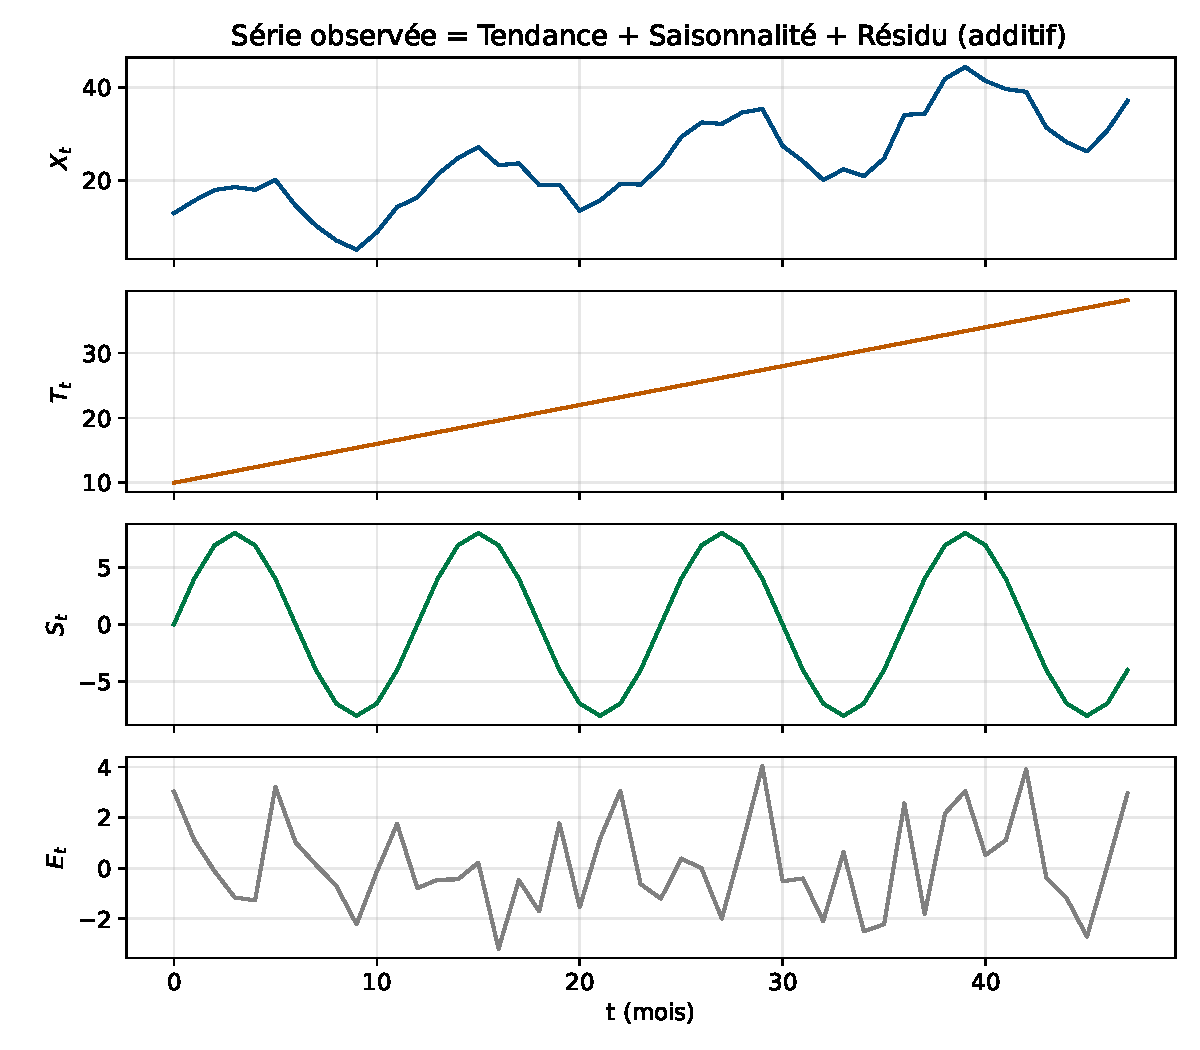
\includegraphics[width=0.82\textwidth]{decomposition.pdf}
\caption{Décomposition additive d'une série : $X_t=T_t+S_t+E_t$ (tendance linéaire,
saisonnalité de période 12, bruit).}
\end{figure}
\begin{lecture}[modèle additif ou multiplicatif ?]
On trace mentalement la droite des maxima et celle des minima. Si l'écart entre les deux
reste \emph{constant} (droites parallèles) $\Rightarrow$ \textbf{additif}. Si l'écart
\emph{croît avec le niveau} (droites divergentes) $\Rightarrow$ \textbf{multiplicatif}.
Sur la figure d'identification (Q\,I.1), comparer les panneaux (3) additif et (4)
multiplicatif : dans (4) l'amplitude des oscillations augmente avec le niveau.
\end{lecture}

\section{Estimation de la tendance par moyennes mobiles}
\begin{definition}[Moyenne mobile]
Une \emph{moyenne mobile} (MM) est un \textbf{filtre linéaire}
$M(X)_t=\sum_{i=-m_1}^{m_2}\lambda_i X_{t-i}$. Elle est \emph{centrée} si $m_1=m_2$,
\emph{symétrique} si $\lambda_{-i}=\lambda_i$, \emph{normalisée} si $\sum_i\lambda_i=1$.
\end{definition}
\begin{attention}[$\to$ Q\,A.2]
Une MM est \emph{par définition} linéaire ; elle n'est \emph{pas} forcément centrée,
symétrique ou normalisée. La bonne réponse au QCM est donc « filtre linéaire, pas forcément
centré ou symétrique ».
\end{attention}
\begin{definition}[MM centrée d'ordre $p$]
Pour absorber une saisonnalité de période $p$ :
si $p$ \emph{impair}, $\mathrm{MM}_p(X)_t=\frac1p\sum_{i=-(p-1)/2}^{(p-1)/2}X_{t-i}$ ;
si $p$ \emph{pair}, on centre en pondérant les bords par $\tfrac12$, ex.
\[
\mathrm{MM}_4(X)_t=\tfrac18X_{t-2}+\tfrac14X_{t-1}+\tfrac14X_t+\tfrac14X_{t+1}+\tfrac18X_{t+2}.
\]
\end{definition}
\begin{theoreme}[Propriétés d'une MM d'ordre $p$]\label{th:mm}
La MM centrée d'ordre $p$ :
\emph{(i)} laisse \textbf{invariante} une tendance affine $T_t=\alpha+\beta t$ ;
\emph{(ii)} \textbf{annule} une saisonnalité de période $p$ (de somme nulle sur une période) ;
\emph{(iii)} \textbf{réduit} la variance du bruit.
\end{theoreme}
\begin{proof}
\emph{(i)} Pour $p$ impair, $\frac1p\sum_{i=-m}^{m}\big(\alpha+\beta(t-i)\big)
=\alpha+\beta t-\frac{\beta}{p}\sum_{i=-m}^{m}i=\alpha+\beta t$ (la somme des $i$ symétriques
est nulle). Pour $p$ pair, le même calcul avec les poids $\tfrac12$ aux bords redonne
$\alpha+\beta t$.
\emph{(ii)} Si $S_t$ est de période $p$ et $\sum_{j=1}^{p}S_j=0$, la moyenne sur une fenêtre
couvrant exactement une période vaut $\frac1p\sum_{j=1}^pS_j=0$.
\emph{(iii)} Si $E_t\sim\BB(0,\sigma^2)$, $\Var\big(\frac1p\sum E_{t-i}\big)=\sigma^2/p<\sigma^2$.
\end{proof}
\begin{figure}[h]
\centering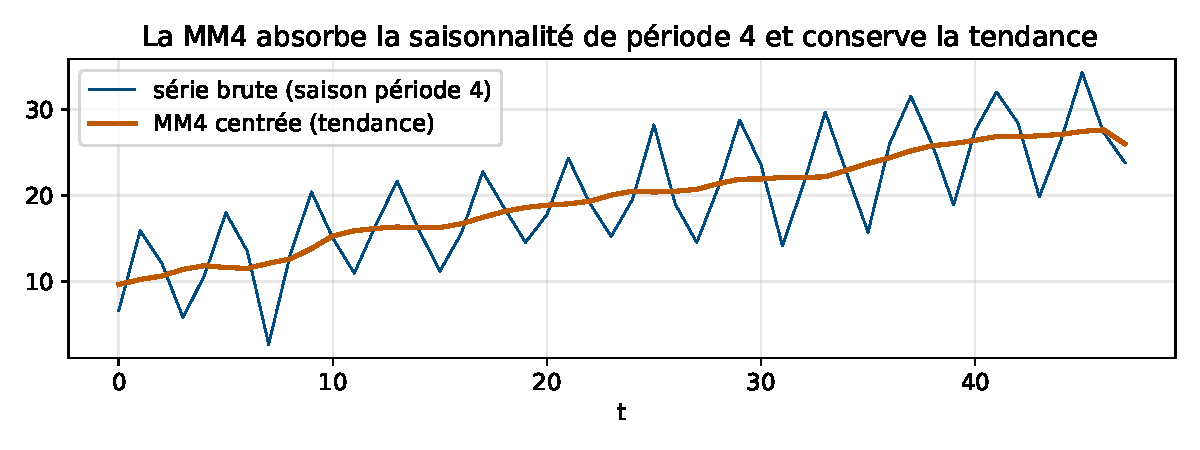
\includegraphics[width=0.78\textwidth]{mm4.pdf}
\caption{La MM4 centrée appliquée à une série trimestrielle : elle gomme la saisonnalité
de période 4 et restitue la tendance.}
\end{figure}
\begin{recette}[$\to$ Q\,A.3]
\textbf{La MM$_p$ absorbe la saisonnalité de période $p$ et conserve une tendance linéaire.}
En particulier la \textbf{MM4} \emph{conserve les tendances linéaires} et \emph{absorbe les
saisonnalités de période 4}. Pour une série de période $p$, on extrait la tendance par
$\mathrm{MM}_p$.
\end{recette}

\section{Coefficients saisonniers et désaisonnalisation}
\begin{methode}[Coefficients saisonniers et série CVS]
\begin{enumerate}[leftmargin=*,nosep]
\item Estimer $T_t$ (par $\mathrm{MM}_p$ ou par régression linéaire $\hat T_t=\hat a t+\hat b$).
\item \emph{Données sans tendance} : $Y_t-T_t$ (additif) ou $Y_t/T_t$ (multiplicatif).
\item Pour chaque saison $j=1,\dots,p$ : $S_j=$ moyenne des données sans tendance de la saison $j$.
\item \textbf{Correction (conservation des aires)} : la moyenne des $S_j$ doit valoir $0$
(additif) ou $1$ (multiplicatif). On pose $S_j'=S_j-\bar S$ (additif) ou $S_j'=S_j/\bar S$
(multiplicatif).
\item \emph{Série CVS} : $\text{CVS}_t=Y_t-S'_{j(t)}$ (additif) ou $Y_t/S'_{j(t)}$ (multiplicatif).
\item \emph{Prévision} : $\widehat X_t=\hat T_t+S'_{j(t)}$ (additif) ou $\hat T_t\,S'_{j(t)}$.
\end{enumerate}
\end{methode}
\begin{recette}[Régression de la tendance ; $\to$ Q\,H.1, H.4]
$\hat a=\dfrac{n\sum tY-\sum t\sum Y}{n\sum t^2-(\sum t)^2}$, $\hat b=\bar Y-\hat a\bar t$.
La prévision linéaire en $t_0$ est $\hat a\,t_0+\hat b$.
\end{recette}

\section{Élimination de la tendance par différenciation}
\begin{definition}
$\Delta X_t=(1-B)X_t=X_t-X_{t-1}$ ; $\Delta^2X_t=(1-B)^2X_t$.
\end{definition}
\begin{proposition}\label{prop:diff}
Si $X_t=\alpha+\beta t+e_t$ (tendance linéaire) alors $\Delta X_t=\beta+\Delta e_t$.
Si $X_t=\alpha+\beta t+\delta t^2+e_t$ alors $\Delta^2X_t=2\delta+\Delta^2e_t$.
\end{proposition}
\begin{proof}
$\Delta(\alpha+\beta t)=\beta$ ; $\Delta(\delta t^2)=\delta(t^2-(t-1)^2)=\delta(2t-1)$, puis
$\Delta^2(\delta t^2)=\delta\big[(2t-1)-(2t-3)\big]=2\delta$.
\end{proof}
La différenciation est l'outil pour stationnariser une tendance \emph{stochastique}
(chapitre 4) ; on ne l'applique qu'après diagnostic (test de racine unité).

\begin{remarque}[Sur les lissages, $\to$ Q\,A.7, A.8]
Le \emph{lissage exponentiel simple} ajuste localement une \emph{constante} (ne capte ni
tendance ni saison). Le lissage double (Holt) capte la tendance ; le lissage de
\emph{Holt--Winters} capte tendance \emph{et} saisonnalité. L'algorithme \emph{X11} estime la
série CVS de façon itérative en combinant régressions et moyennes mobiles ($\to$ Q\,A.4).
\end{remarque}

% ====================================================================
\chapter{Processus stationnaires au sens large}

\section{Définition et fonction d'autocorrélation}
\begin{definition}[Stationnarité au sens large, SSL]
$(X_t)$ est \emph{SSL} (ou du second ordre) si :
(i) $\E(X_t)=m$ constante ; (ii) $\E(X_t^2)<\infty$ ;
(iii) $\gamma(k)=\Cov(X_t,X_{t+k})$ ne dépend que de $k$. On note
$\gamma(0)=\Var(X_t)$ et $\rho(k)=\gamma(k)/\gamma(0)$ (ACF).
\end{definition}
\begin{proposition}[Propriétés de $\gamma$ et $\rho$]
$\gamma(-k)=\gamma(k)$ ; $|\gamma(k)|\le\gamma(0)$ ; $\rho(0)=1$ ; $|\rho(k)|\le1$.
\end{proposition}
\begin{proof}
Parité : $\gamma(-k)=\Cov(X_t,X_{t-k})=\Cov(X_{t-k},X_t)=\gamma(k)$ (par stationnarité, on
décale de $k$). L'inégalité $|\gamma(k)|\le\gamma(0)$ découle de Cauchy--Schwarz :
$|\Cov(X_t,X_{t+k})|\le\sqrt{\Var(X_t)\Var(X_{t+k})}=\gamma(0)$.
\end{proof}
\begin{definition}[Stationnarité stricte]
$(X_t)$ est \emph{strictement stationnaire} si la loi de $(X_{t_1},\dots,X_{t_n})$ est
invariante par translation. Si de plus $\E(X_t^2)<\infty$, alors strict $\Rightarrow$ SSL.
\end{definition}
\begin{recette}[$\to$ Q\,A.15, A.16]
\textbf{SSL} ne porte que sur les \emph{deux premiers moments} (donc vérifiable) ; la
stationnarité \emph{stricte} porte sur toute la loi. Strict $+$ carré intégrable
$\Rightarrow$ SSL.
\end{recette}

\section{Le bruit blanc}
\begin{definition}[Bruit blanc]
$(a_t)\sim\BB(0,\sigma^2)$ si $\E(a_t)=0$, $\Var(a_t)=\sigma^2$, $\gamma(k)=0$ pour $k\ne0$.
\emph{Fort} si les $a_t$ sont i.i.d. ; \emph{faible} s'ils sont seulement non corrélés ;
\emph{gaussien} si i.i.d.\ $N(0,\sigma^2)$.
\end{definition}
\begin{exemple}[$X_t=a_t-a_{t-1}$]
$\E(X_t)=0$ ; $\gamma(0)=\Var(a_t)+\Var(a_{t-1})=2\sigma^2$ ;
$\gamma(1)=\Cov(a_t-a_{t-1},a_{t-1}-a_{t-2})=-\sigma^2$ ; $\gamma(k)=0$ ($k\ge2$).
Indépendant de $t$ : $X_t$ est SSL.
\end{exemple}
\begin{exemple}[Le processus $X_t=(-1)^t z$ ; $\to$ Q\,B.1]
Soit $z$ avec $\E(z)=0$, $\Var(z)=1$. Alors $\E(X_t)=(-1)^t\E(z)=0$ et
\[
\gamma(k)=\Cov\big((-1)^tz,(-1)^{t+k}z\big)=(-1)^{2t+k}\E(z^2)=(-1)^k,
\]
\emph{indépendant de $t$}. Donc $(X_t)$ est \textbf{SSL}, avec $\gamma(0)=1$ et
$\rho(k)=(-1)^k$.
\end{exemple}

\section{Non-stationnarité : processus TS et DS, intégration}
\begin{definition}[TS, \emph{trend stationary}]
$(X_t)$ est TS s'il s'écrit $X_t=f(t)+Z_t$, $f$ déterministe (ex.\ $f(t)=\alpha+\beta t$),
$Z_t$ stationnaire. On le rend stationnaire en \emph{retranchant la tendance}.
\end{definition}
\begin{definition}[DS / intégration]
$(X_t)$ est \emph{intégré d'ordre $d$}, $X_t\sim I(d)$, si $(1-B)^dX_t$ est stationnaire et
$d$ est minimal. Pour $d=1$ : $(1-B)X_t$ stationnaire $\iff X_t=X_{t-1}+Z_t$ (DS).
\end{definition}
\begin{theoreme}[La marche aléatoire est non stationnaire]
Soit $X_t=X_{t-1}+a_t$ (i.e.\ $(1-B)X_t=a_t$), $X_0$ fixé. Alors
$X_t=X_0+\sum_{j=1}^t a_j$, donc $\Var(X_t)=t\sigma^2\to\infty$ : $(X_t)$ n'est pas SSL,
$X_t\sim I(1)$.
\end{theoreme}
\begin{proof}
Par récurrence $X_t=X_0+a_1+\dots+a_t$ ; les $a_j$ étant non corrélés,
$\Var(X_t)=\sum_{j=1}^t\sigma^2=t\sigma^2$ dépend de $t$.
\end{proof}
\begin{figure}[h]
\centering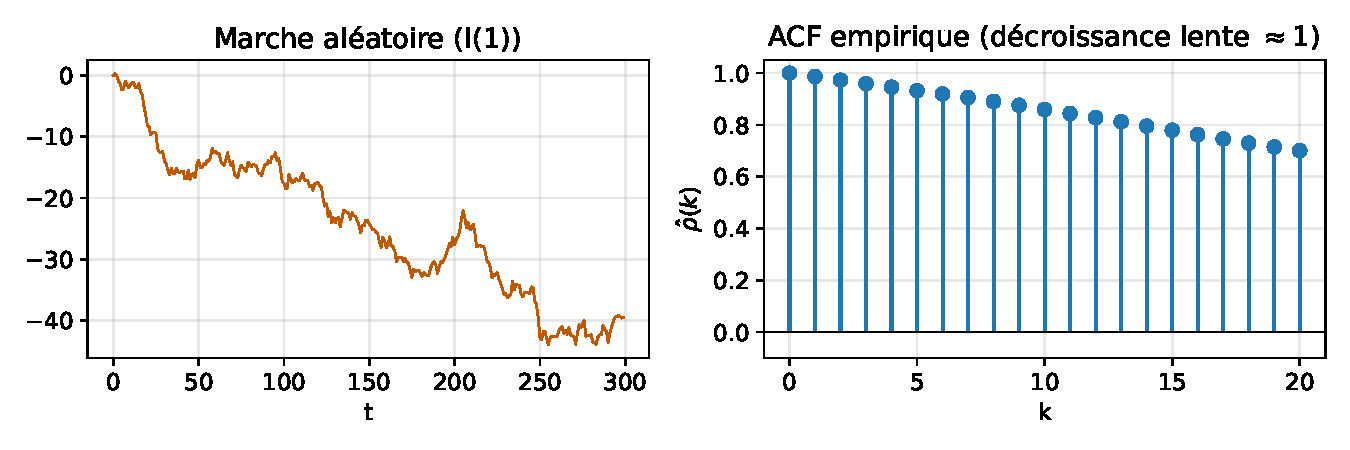
\includegraphics[width=0.92\textwidth]{nonstat.pdf}
\caption{Marche aléatoire $I(1)$ (gauche) et son ACF empirique (droite) :
décroissance \emph{très lente} caractéristique de la non-stationnarité.}
\end{figure}
\begin{lecture}[reconnaître une non-stationnarité]
Une série non stationnaire a une ACF empirique qui \textbf{décroît très lentement}
($\rhohat(1)\approx1$). Une série stationnaire a une ACF qui \textbf{décroît rapidement vers
0}. C'est le premier diagnostic visuel ($\to$ tests de Dickey--Fuller, ch.~4).
\end{lecture}
\begin{attention}[$\to$ Q\,A.14 ; Q\,F.4(e)]
\emph{Stationnaire $\ne$ bruit blanc} : un AR(1) est stationnaire mais fortement autocorrélé.
On ne stationnarise un \emph{TS} qu'en retranchant la tendance, un \emph{DS} qu'en
différenciant ; \emph{sur-différencier} une série stationnaire \emph{augmente} la variance.
\end{attention}

% ====================================================================
\chapter{Modèles ARMA}

\section{Écriture polynomiale}
Le modèle linéaire général
$X_t=\mu+\sum_{i=1}^p\phi_iX_{t-i}+a_t-\sum_{j=1}^q\theta_ja_{t-j}$ s'écrit
$\Phi_p(B)X_t=\mu+\Theta_q(B)a_t$, avec
$\Phi_p(B)=1-\phi_1B-\dots-\phi_pB^p$ et $\Theta_q(B)=1-\theta_1B-\dots-\theta_qB^q$.

\section{Processus moyenne mobile MA$(q)$}
\begin{definition}
$X_t=\mu+a_t+\theta_1a_{t-1}+\dots+\theta_qa_{t-q}$, $a_t\sim\BB(0,\sigma^2)$.
\end{definition}
\begin{theoreme}[Moments du MA$(q)$]\label{th:maq}
$\E(X_t)=\mu$ et
\[
\gamma(k)=\begin{cases}
\big(1+\theta_1^2+\dots+\theta_q^2\big)\sigma^2,&k=0,\\
\sigma^2\big(\theta_k+\sum_{j=1}^{q-k}\theta_j\theta_{k+j}\big),&1\le k\le q,\\
0,&k>q,
\end{cases}\qquad(\theta_0:=1).
\]
\emph{Tout MA$(q)$ est SSL.}
\end{theoreme}
\begin{proof}
Posons $Y_t=X_t-\mu=\sum_{i=0}^q\theta_i a_{t-i}$. Comme $\Cov(a_{t-i},a_{t+k-j})=\sigma^2$
ssi $t-i=t+k-j$, i.e.\ $j=i+k$, on a
$\gamma(k)=\Cov(Y_t,Y_{t+k})=\sum_{i,j}\theta_i\theta_j\Cov(a_{t-i},a_{t+k-j})
=\sigma^2\sum_{i}\theta_i\theta_{i+k}$, la somme portant sur $0\le i,\ i+k\le q$. Pour $k=0$
on retrouve $\sigma^2\sum_i\theta_i^2$ ; pour $k>q$ la somme est vide, $\gamma(k)=0$.
Comme $\gamma(k)$ ne dépend pas de $t$ et $\E(X_t)=\mu$, $X_t$ est SSL.
\end{proof}
\begin{corollaire}[ACF du MA$(q)$ : coupure à $q$]
$\rho(k)\ne0$ pour $0\le k\le q$ et $\rho(k)=0$ pour $k>q$.
\end{corollaire}
\begin{exemple}[MA(1)]
$X_t=\mu+a_t+\theta a_{t-1}$ : $\gamma(0)=(1+\theta^2)\sigma^2$, $\gamma(1)=\theta\sigma^2$,
$\gamma(k)=0$ ($k\ge2$), donc $\rho(1)=\dfrac{\theta}{1+\theta^2}$, $\rho(k)=0$ ($k\ge2$).
\end{exemple}
\begin{figure}[h]
\centering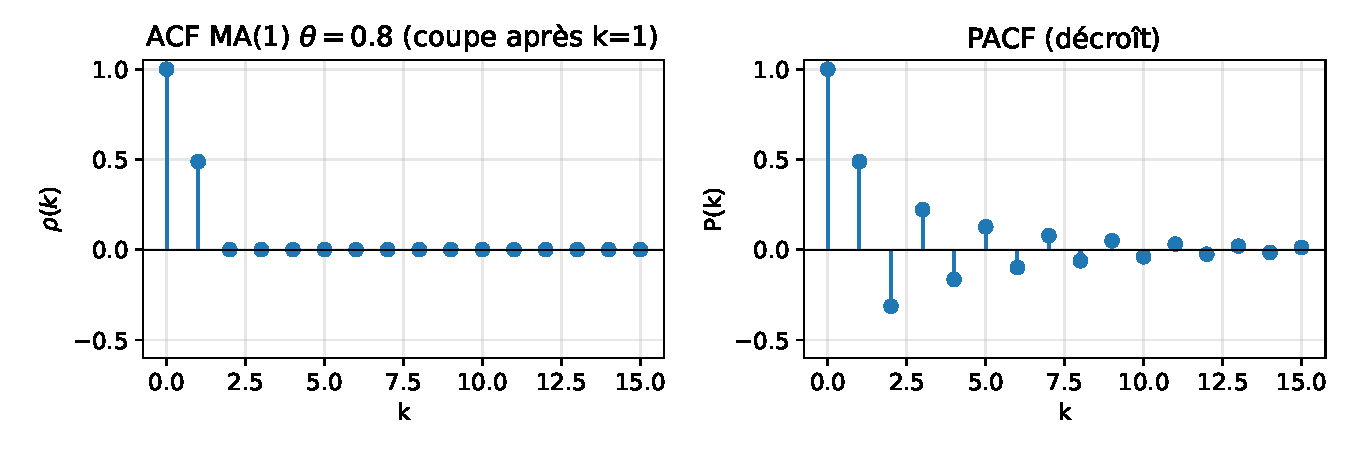
\includegraphics[width=0.92\textwidth]{acfpacf_ma1.pdf}
\caption{MA(1), $\theta=0.8$ : l'ACF \textbf{coupe après $k=1$}, la PACF \textbf{décroît}
(dualité avec l'AR).}
\end{figure}

\section{Inversibilité et représentation AR$(\infty)$}
\begin{definition}[Inversibilité]
Un MA$(q)$ est \emph{inversible} si les racines de $\Theta_q(B)=0$ sont de module $>1$ ; on
peut alors écrire $a_t=\Theta_q(B)^{-1}X_t$ (forme $\mathrm{AR}(\infty)$).
\end{definition}
\begin{exemple}
$X_t=(1-\theta B)a_t$ avec $|\theta|<1$ : $(1-\theta B)^{-1}=\sum_{i\ge0}\theta^iB^i$ converge,
d'où $a_t=\sum_{i\ge0}\theta^iX_{t-i}$.
\end{exemple}
\begin{attention}[$\to$ Q\,A.12]
Tout MA est \emph{stationnaire} mais n'admet une représentation AR que s'il est
\emph{inversible}. Contre-exemple : $X_t=a_t-a_{t-1}$ (racine $B=1$) non inversible.
\end{attention}

\section{Processus autorégressif AR$(p)$}
\begin{definition}
$X_t=\mu+\phi_1X_{t-1}+\dots+\phi_pX_{t-p}+a_t$, $\phi_p\ne0$.
\end{definition}
\begin{theoreme}[Stationnarité et causalité]\label{th:arp}
L'AR$(p)$ $\Phi_p(B)X_t=\mu+a_t$ est SSL et \emph{causal} \textbf{ssi toutes les racines de
$\Phi_p(B)=0$ sont de module strictement $>1$}. Il admet alors la forme causale
$X_t=\dfrac{\mu}{1-\sum\phi_i}+\sum_{j\ge0}\psi_j a_{t-j}$ avec $\psi_0=1$, $\sum_j\psi_j^2<\infty$.
\end{theoreme}
\begin{proof}[Cas AR(1), entièrement détaillé]
$(1-\phi B)X_t=\mu+a_t$.
\emph{($\Leftarrow$)} Si $|\phi|<1$, la série $\sum_{k\ge0}\phi^kB^k$ converge et inverse
$(1-\phi B)$, donc
$X_t=\dfrac{\mu}{1-\phi}+\sum_{k\ge0}\phi^k a_{t-k}$, avec $\sum\phi^{2k}=\frac1{1-\phi^2}<\infty$.
\emph{($\Rightarrow$)} Si $\phi=1$, alors $X_t=X_0+t\mu+\sum_{j=1}^t a_j$ et
$\Var(X_t)=t\sigma^2\to\infty$ : non SSL. Plus généralement, la racine de $1-\phi B$ est
$B=1/\phi$, de module $>1$ ssi $|\phi|<1$.
\end{proof}
\begin{theoreme}[Démonstration pour l'AR(2)]
Soit $\Phi(B)=1-\phi_1B-\phi_2B^2=(1-\tfrac{B}{b_1})(1-\tfrac{B}{b_2})$, $b_1,b_2$ racines.
Posons $Y_t=(1-\tfrac{B}{b_2})X_t$ ; alors $(1-\tfrac{B}{b_1})Y_t=\mu+a_t$ est un AR(1) de
paramètre $1/b_1$, stationnaire ssi $|b_1|>1$. En réinjectant, $X_t$ est stationnaire causal
ssi $|b_1|>1$ et $|b_2|>1$, et
$X_t=\dfrac{\mu}{1-\phi_1-\phi_2}+\sum_{j\ge0}\psi_j a_{t-j}$.
\end{theoreme}
\begin{corollaire}[Moments de l'AR(1) causal, $|\phi|<1$]\label{cor:ar1}
\[
\E(X_t)=\frac{\mu}{1-\phi},\quad \Var(X_t)=\frac{\sigma^2}{1-\phi^2},\quad
\gamma(k)=\frac{\sigma^2}{1-\phi^2}\phi^{|k|},\quad \rho(k)=\phi^{|k|}.
\]
\end{corollaire}
\begin{proof}
Causalité $\Rightarrow\Cov(a_t,X_{t-1})=0$. D'où
$\Var(X_t)=\phi^2\Var(X_{t-1})+\sigma^2\Rightarrow\gamma(0)=\sigma^2/(1-\phi^2)$.
Puis $\gamma(k)=\Cov(X_t,\phi X_{t+k-1}+\mu+a_{t+k})=\phi\gamma(k-1)$ pour $k\ge1$, donc
$\gamma(k)=\phi^k\gamma(0)$ et $\rho(k)=\phi^k$.
\end{proof}
\begin{figure}[h]
\centering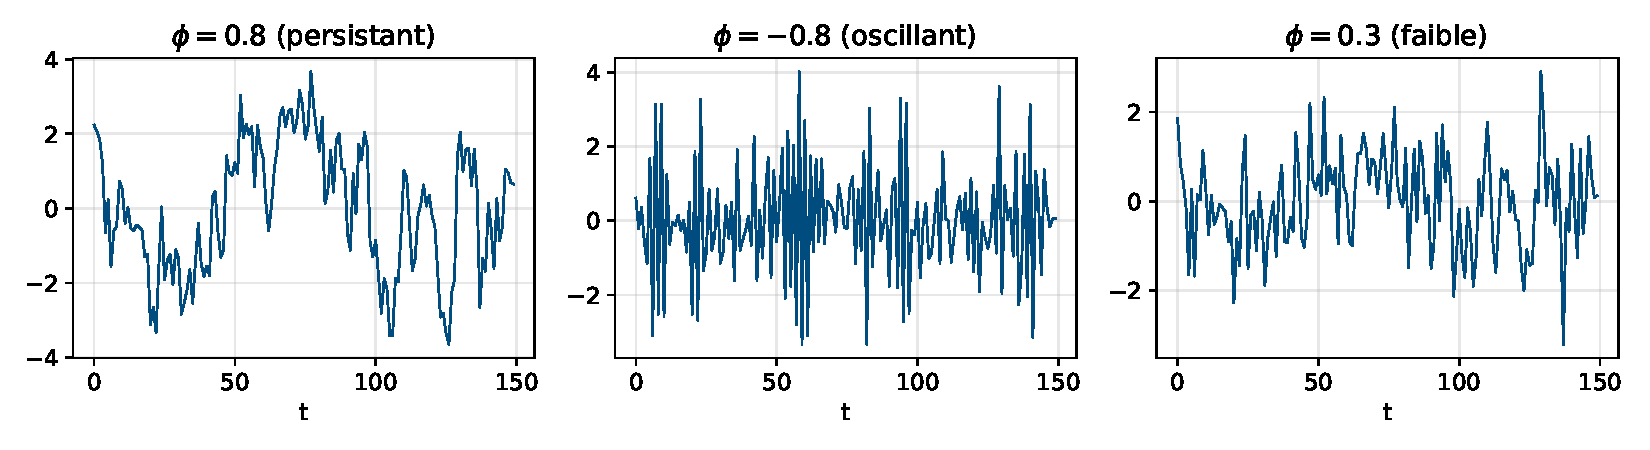
\includegraphics[width=0.97\textwidth]{ar1_traj.pdf}
\caption{Trajectoires d'AR(1) : forte persistance ($\phi=0.8$), alternance de signe
($\phi=-0.8$), quasi-bruit ($\phi=0.3$).}
\end{figure}
\begin{figure}[h]
\centering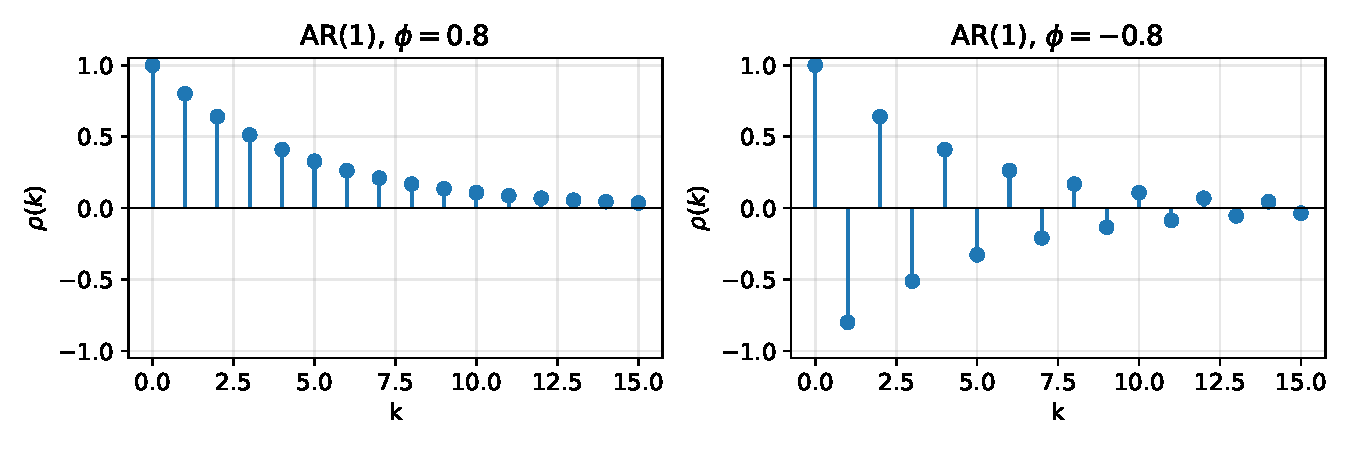
\includegraphics[width=0.82\textwidth]{acf_ar1.pdf}
\caption{ACF d'un AR(1) : décroissance géométrique $\rho(k)=\phi^k$ (monotone si $\phi>0$,
oscillante si $\phi<0$).}
\end{figure}
\begin{lecture}[reconnaître un AR(1) sur le graphe]
$\phi>0$ : trajectoire \emph{lisse et persistante}, ACF qui décroît en restant positive.
$\phi<0$ : trajectoire \emph{en dents de scie}, ACF \emph{alternée} ($+,-,+,\dots$). Plus
$|\phi|$ est proche de 1, plus la mémoire (et la décroissance lente de l'ACF) est forte.
\end{lecture}

\section{Équations de Yule--Walker}
\begin{theoreme}[Yule--Walker]\label{th:yw}
Pour un AR$(p)$ SSL causal,
\[
\rho(k)=\sum_{j=1}^p\phi_j\,\rho(k-j)\ (k\ge1),\qquad
\gamma(0)=\frac{\sigma^2}{1-\sum_{j=1}^p\phi_j\rho(j)}.
\]
Cas AR(2) : $\rho(1)=\dfrac{\phi_1}{1-\phi_2}$, $\rho(2)=\phi_1\rho(1)+\phi_2$.
\end{theoreme}
\begin{proof}
Pour $k\ge1$ : $\gamma(k)=\Cov\big(X_{t-k},\sum_j\phi_jX_{t-j}+\mu+a_t\big)
=\sum_j\phi_j\gamma(k-j)$ car $\Cov(X_{t-k},a_t)=0$ ($k\ge1$, causalité). Diviser par
$\gamma(0)$ donne la récurrence. Pour $k=0$ :
$\gamma(0)=\sum_j\phi_j\gamma(j)+\Cov(X_t,a_t)=\sum_j\phi_j\gamma(j)+\sigma^2$, d'où
$\gamma(0)$. Pour l'AR(2), $k=1$ : $\rho(1)=\phi_1+\phi_2\rho(1)$ (car $\rho(-1)=\rho(1)$),
soit $\rho(1)=\phi_1/(1-\phi_2)$ ; $k=2$ : $\rho(2)=\phi_1\rho(1)+\phi_2$.
\end{proof}
\begin{recette}[Estimation par Yule--Walker ; $\to$ Q\,G.1--G.3, J.16]
On résout $\boldsymbol\rho=R\,\boldsymbol\phi\Rightarrow\boldsymbol\phi=R^{-1}\boldsymbol\rho$,
puis $\hat\sigma^2=\gamma(0)\big(1-\sum\phi_j\rho(j)\big)$. AR(1) : $\hat\phi=\rhohat(1)$ ;
AR(2) : $\hat\phi_1=\dfrac{\rho_1(1-\rho_2)}{1-\rho_1^2}$,
$\hat\phi_2=\dfrac{\rho_2-\rho_1^2}{1-\rho_1^2}$.
\end{recette}

\section{Fonction d'autocorrélation partielle (FAP)}
\begin{definition}[FAP]
$P(k)$ est la corrélation entre $X_t$ et $X_{t+k}$ \emph{après élimination de l'effet linéaire}
des variables intermédiaires. On a $P(1)=\rho(1)$ et, par la formule matricielle de
Yule--Walker tronquée,
\[
P(2)=\frac{\begin{vmatrix}1&\rho_1\\ \rho_1&\rho_2\end{vmatrix}}
{\begin{vmatrix}1&\rho_1\\ \rho_1&1\end{vmatrix}}
=\frac{\rho_2-\rho_1^2}{1-\rho_1^2}.
\]
\end{definition}
\begin{theoreme}[FAP d'un AR$(p)$ : coupure à $p$]\label{th:pacf}
Pour un AR$(p)$ : $P(k)=0$ pour $k>p$, et $P(p)=\phi_p$.
\end{theoreme}
\begin{proof}[Idée]
La projection de $X_t$ sur $X_{t-1},\dots,X_{t-k}$ a pour dernier coefficient $\phi_{kk}$
solution de Yule--Walker à l'ordre $k$. Pour $k>p$, le modèle exact n'utilise que $p$ retards,
donc $\phi_{kk}=0$ ; pour $k=p$, $\phi_{pp}=\phi_p$.
\end{proof}
\begin{theoreme}[Dualité AR / MA]\label{th:dual}
\begin{center}\renewcommand{\arraystretch}{1.2}
\begin{tabular}{lll}
\toprule
& \textbf{ACF} ($\rho$) & \textbf{FAP} ($P$)\\\midrule
\textbf{AR$(p)$} & décroît (exp.\ /sinus amortie) & \textbf{nulle pour $k>p$}\\
\textbf{MA$(q)$} & \textbf{nulle pour $k>q$} & décroît\\
\textbf{ARMA$(p,q)$} & décroît & décroît\\
\bottomrule
\end{tabular}
\end{center}
\end{theoreme}
\begin{figure}[h]
\centering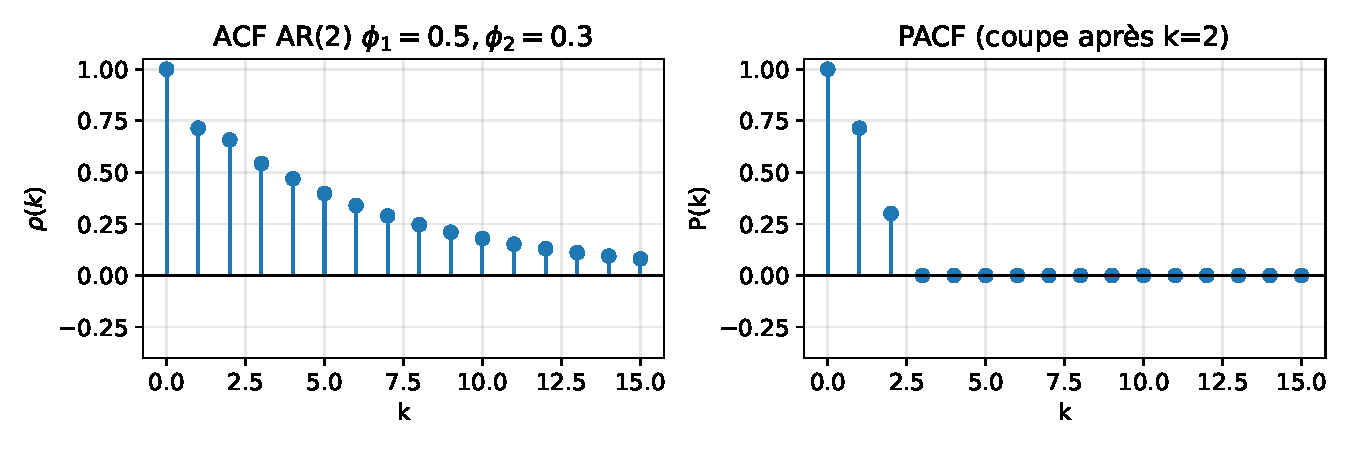
\includegraphics[width=0.92\textwidth]{acfpacf_ar2.pdf}
\caption{AR(2), $\phi_1=0.5,\phi_2=0.3$ : l'ACF \textbf{décroît}, la PACF \textbf{coupe après
$k=2$} ($P(2)=\phi_2$).}
\end{figure}
\begin{recette}[Identifier $p$ et $q$ ; $\to$ Q\,A.9, A.10, D.5, I.2, I.3]
\textbf{FAP coupe à $p$ et ACF décroît} $\Rightarrow$ AR$(p)$.
\textbf{ACF coupe à $q$ et FAP décroît} $\Rightarrow$ MA$(q)$.
\textbf{Les deux décroissent} $\Rightarrow$ ARMA. Bande de non-significativité $\pm2/\sqrt n$.
\end{recette}

\section{Modèle ARMA$(p,q)$ et représentations infinies}
\begin{definition}
$\Phi_p(B)X_t=\mu+\Theta_q(B)a_t$ : \emph{stationnaire/causal} ssi racines de $\Phi_p$ de
module $>1$ ; \emph{inversible} ssi racines de $\Theta_q$ de module $>1$. Alors
$\E(X_t)=\mu/(1-\phi_1-\dots-\phi_p)$.
\end{definition}
\begin{theoreme}[Coefficients $\psi_k$ (MA$\infty$) et $\pi_k$ (AR$\infty$)]\label{th:repr}
\begin{itemize}[leftmargin=*,nosep]
\item Forme $\mathrm{MA}(\infty)$ $X_t=\sum_k\psi_ka_{t-k}$ : $\Phi(B)\Psi(B)=\Theta(B)$, d'où
$\psi_k=\theta^\Theta_k+\sum_{j=1}^k\phi_j\psi_{k-j}$ ($\psi_0=1$).
\item Forme $\mathrm{AR}(\infty)$ $a_t=\sum_k\pi_kX_{t-k}$ : $\Theta(B)\Pi(B)=\Phi(B)$, d'où
$\pi_k=\phi^\Phi_k-\sum_{j=1}^k\theta^\Theta_j\pi_{k-j}$ ($\pi_0=1$),
où $\theta^\Theta_j$ (resp.\ $\phi^\Phi_j$) est le coefficient de $B^j$ dans $\Theta$ (resp.\
$\Phi$) ; attention aux signes : $\phi^\Phi_j=-\phi_j$, $\theta^\Theta_j=-\theta_j$.
\end{itemize}
\end{theoreme}
\begin{proof}
Identification des coefficients de $B^k$ dans l'égalité polynomiale $\Phi\Psi=\Theta$ :
$\sum_{j=0}^k\phi^\Phi_j\psi_{k-j}=\theta^\Theta_k$ avec $\phi^\Phi_0=1$, d'où la récurrence
en isolant $\psi_k$. Idem pour $\pi$ via $\Theta\Pi=\Phi$.
\end{proof}
\begin{exemple}[AR(2) $X_t-0.9X_{t-1}+0.2X_{t-2}=a_t$ ; $\to$ Q\,C.1]
$\psi_k=0.9\psi_{k-1}-0.2\psi_{k-2}$ : $\psi_1=0.9,\psi_2=0.61,\psi_3=0.369$. Racines des
inverses $0.5,0.4$, d'où $\psi_k=5(0.5)^k-4(0.4)^k$.
\end{exemple}
\begin{exemple}[$(1-0.8B)X_t=(1+0.4B)a_t$ ; $\to$ Q\,C.3, B.5]
MA$\infty$ : $\psi_k=0.8\psi_{k-1}$, $\psi_1=1.2\Rightarrow\psi_k=1.2(0.8)^{k-1}$.
AR$\infty$ : $\pi_k=-0.4\pi_{k-1}$, $\pi_1=-1.2$.
\end{exemple}
\begin{attention}[Racines communes ; $\to$ Q\,B.3, B.4, J.3]
Si $\Phi$ et $\Theta$ partagent une racine, \textbf{simplifier d'abord}. Ex.\
$(1-1.66B+0.66B^2)=(1-B)(1-0.66B)$ et le second membre $(1-B)a_t$ : le facteur $(1-B)$ se
simplifie, laissant l'AR(1) fini $(1-0.66B)X_t=a_t$.
\end{attention}

\section{Le processus ARMA(1,1) : autocovariance}
\begin{theoreme}[Autocovariances de l'ARMA(1,1)]\label{th:arma11}
Pour $X_t=\phi X_{t-1}+a_t+\theta a_{t-1}$ (stationnaire, $|\phi|<1$) :
\[
\gamma(0)=\sigma^2\frac{1+2\phi\theta+\theta^2}{1-\phi^2},\quad
\gamma(1)=\sigma^2\frac{(1+\phi\theta)(\phi+\theta)}{1-\phi^2},\quad
\gamma(k)=\phi\,\gamma(k-1)\ (k\ge2).
\]
\end{theoreme}
\begin{proof}
On a $\Cov(X_t,a_t)=\sigma^2$ et $\Cov(X_t,a_{t-1})=(\phi+\theta)\sigma^2$ (en multipliant
l'équation par $a_t$, $a_{t-1}$ et en prenant l'espérance, via la causalité). Puis :
$\gamma(0)=\E[X_t(\phi X_{t-1}+a_t+\theta a_{t-1})]
=\phi\gamma(1)+\sigma^2+\theta(\phi+\theta)\sigma^2$ et
$\gamma(1)=\E[X_t(\phi X_t+\dots)]$\dots on résout le système linéaire en $\gamma(0),\gamma(1)$,
ce qui donne les formules. Pour $k\ge2$, l'équation ne fait plus intervenir de terme MA
courant : $\gamma(k)=\phi\gamma(k-1)$.
\end{proof}
\begin{proposition}[Somme de processus indépendants ; $\to$ Q\,D.6, J.18, J.19]
La somme de deux ARMA indépendants ARMA$(p_1,q_1)$ et ARMA$(p_2,q_2)$ est un
ARMA$\big(p_1+p_2,\ \max(p_1+q_2,p_2+q_1)\big)$. En particulier :
\textbf{AR(1) $+$ bruit blanc $=$ ARMA(1,1)} et \textbf{AR(1) $+$ MA(1) $=$ ARMA(1,1)} (après
réduction).
\end{proposition}

% ====================================================================
\chapter{Box--Jenkins : intégration, ARIMA, validation}

\section{Identification par les corrélogrammes}
La démarche de Box--Jenkins : (1) \emph{stationnariser} (différenciation si l'ACF décroît
lentement) ; (2) \emph{identifier} $p,q$ via ACF/PACF (théorème~\ref{th:dual}) ;
(3) \emph{estimer} ; (4) \emph{valider} (résidus $=$ bruit blanc).

\section{Tests de racine unitaire de Dickey--Fuller}
\begin{definition}[DF simple]
On teste la présence d'une racine unité dans un AR(1) via l'un des modèles :
\[
\text{(1) }\Delta X_t=\rho X_{t-1}+\alpha+\beta t+a_t,\quad
\text{(2) }\Delta X_t=\rho X_{t-1}+\alpha+a_t,\quad
\text{(3) }\Delta X_t=\rho X_{t-1}+a_t,
\]
où $\rho=\phi-1$. $H_0:\rho=0$ (i.e.\ $\phi=1$, racine unité, non stationnaire) contre
$H_1:\phi<1$ (AR(1) stationnaire). Statistique
$t_\phi=\dfrac{\hat\phi-1}{\hat\sigma_{\hat\phi}}$, comparée aux valeurs critiques
\emph{de la table de Dickey--Fuller} (et non de Student).
\end{definition}
\begin{methode}[Stratégie et décision]
On part du modèle (1) ; si $\beta$ n'est pas significatif on passe à (2), puis à (3).
\textbf{Décision} : si $t_\phi$ est \emph{supérieur} (moins négatif) à la valeur critique, on
\emph{ne rejette pas} $H_0$ $\Rightarrow$ racine unité $\Rightarrow$ \emph{différencier}.
\end{methode}
\begin{exemple}[$\to$ Q\,F.4]
$\hat\phi=0.996$, $\hat\sigma_{\hat\phi}=0.0061$, $t_\phi=-0.645>-2.89$ : on ne rejette pas
$H_0$, donc $X_t\sim I(1)$. Après différenciation, $\rhohat(1)\approx0$ : $\Delta X_t$ est un
bruit blanc $\Rightarrow$ marche aléatoire, modèle ARIMA$(0,1,0)$.
\end{exemple}
Le test \emph{ADF} (augmenté) étend ceci aux AR$(p)$ en ajoutant des termes
$\sum_j\phi_j\Delta X_{t-j}$.

\section{Processus ARIMA et SARIMA}
\begin{definition}[ARIMA$(p,d,q)$]
Si $X_t\sim I(d)$ et $(1-B)^dX_t$ est un ARMA$(p,q)$ stationnaire :
$\Phi_p(B)(1-B)^dX_t=\Theta_q(B)a_t$. Cas : ARIMA$(p,0,q)=$ARMA$(p,q)$ ;
ARIMA$(0,1,0)=$ marche aléatoire.
\end{definition}
\begin{recette}[Trouver $(p,d,q)$ ; $\to$ Q\,F.1, F.2, F.3, J.13]
\textbf{1.} Tester $\Phi(1)=0$ (c.-à-d.\ $\sum\phi_i=1$) et factoriser $(1-B)$ autant que
possible $\to d$. \textbf{2.} Le polynôme stationnaire restant donne $p$ ; le polynôme MA
donne $q$.
\end{recette}
\begin{exemple}[$\to$ Q\,F.1]
$1-2.65B+2.3B^2-0.65B^3=(1-B)^2(1-0.65B)$ (deux racines unités) $\Rightarrow X_t\sim I(2)$,
ARIMA$(1,2,0)$.
\end{exemple}
\begin{definition}[SARIMA]
$\Phi_p(B)\Phi_P(B^s)(1-B)^d(1-B^s)^DX_t=\Theta_q(B)\Theta_Q(B^s)a_t$ : il modélise
\emph{tendance et/ou saisonnalité} (période $s$). $\to$ Q\,A.11, I.3.
\end{definition}

\section{Validation : test de Ljung--Box}
\begin{definition}[Statistique de Ljung--Box]
Après ajustement d'un ARMA$(p,q)$, on teste la \emph{blancheur des résidus} :
\[
\mathrm{LB}=n(n+2)\sum_{k=1}^{K}\frac{\rhohat_k^2}{n-k}\ \xrightarrow{H_0}\ \chi^2_{K-p-q},
\]
$H_0$ : « résidus $=$ bruit blanc ». On \textbf{rejette $H_0$} si
$\mathrm{LB}>\chi^2_{K-p-q,\,1-\alpha}$.
\end{definition}
\begin{exemple}[$\to$ Q\,J.21]
ARMA(1,1), $K=14$ : ddl $=14-1-1=12$, $\chi^2_{12,0.95}=21.03$. Si $\mathrm{LB}=18.386<21.03$,
on \emph{ne rejette pas} $H_0$ : résidus compatibles avec un bruit blanc, modèle validé.
\end{exemple}
\begin{recette}[Validation complète ; $\to$ Q\,A.13, A.19--A.21]
(i) significativité des paramètres (Student) ; (ii) \textbf{blancheur des résidus}
(Ljung--Box, ACF/PACF des résidus) ; (iii) normalité (Jarque--Bera). \emph{Sélection} :
\textbf{AIC}$=-2\ln L+2k$, \textbf{BIC}$=-2\ln L+k\ln n$ (on \emph{minimise}).
\end{recette}

% ====================================================================
\chapter{Prévision}

\section{Prévision optimale et règles de calcul}
\begin{definition}
La meilleure prévision (au sens de l'erreur quadratique moyenne) de $X_{n+h}$ connaissant le
passé est $\widehat X_{n+h}=\E[X_{n+h}\mid\mathcal F_n]$.
\end{definition}
\begin{methode}[Calcul]
Écrire l'équation à la date $n+h$ ; remplacer les chocs \emph{futurs} $a_{n+j}$ ($j\ge1$)
par $0$, les chocs \emph{passés} par les résidus, et les $X$ futurs par leurs prévisions.
\end{methode}

\section{Prévision d'un AR$(p)$ et d'un MA(1)}
\begin{theoreme}[AR$(p)$]
$\widehat X_{n+h}=\mu+\sum_{j=1}^p\phi_j\widehat X_{n+h-j}$ (avec $\widehat X_{n+i}=X_{n+i}$
pour $i\le0$). En particulier AR(1) :
$\widehat X_{n+h}=\phi^hX_n+\mu\sum_{j=0}^{h-1}\phi^j\xrightarrow{h\to\infty}\dfrac{\mu}{1-\phi}$.
\end{theoreme}
\begin{theoreme}[MA(1)]
$\widehat X_{n+1}=\mu+\theta a_n$, et $\widehat X_{n+h}=\mu$ pour $h\ge2$ (au-delà de
l'horizon $q$, un MA$(q)$ prévoit sa moyenne).
\end{theoreme}

\section{Erreur de prévision et intervalle de confiance}
\begin{theoreme}[Erreur de prévision]\label{th:err}
Via la forme $\mathrm{MA}(\infty)$ $X_t=\mu+\sum_j\psi_ja_{t-j}$,
\[
\Delta_h=X_{n+h}-\widehat X_{n+h}=\sum_{j=0}^{h-1}\psi_j a_{n+h-j},\qquad
\Var(\Delta_h)=\sigma^2\sum_{j=0}^{h-1}\psi_j^2.
\]
\end{theoreme}
\begin{proof}[Cas AR(1)]
En itérant $X_{n+h}=\mu\sum_{j=0}^{h-1}\phi^j+\phi^hX_n+\sum_{j=0}^{h-1}\phi^j a_{n+h-j}$.
Or $\widehat X_{n+h}=\mu\sum_{j=0}^{h-1}\phi^j+\phi^hX_n$ (chocs futurs nuls), d'où
$\Delta_h=\sum_{j=0}^{h-1}\phi^j a_{n+h-j}$ et
$\Var(\Delta_h)=\sigma^2\sum_{j=0}^{h-1}\phi^{2j}$.
\end{proof}
\begin{corollaire}
AR(1) : $\Var(\Delta_h)=\sigma^2(1+\phi^2+\dots+\phi^{2(h-1)})$.\quad
MA(1) : $\Var(\Delta_1)=\sigma^2$, $\Var(\Delta_h)=(1+\theta^2)\sigma^2$ ($h\ge2$).
\end{corollaire}
\begin{theoreme}[Intervalle de confiance]
Sous $a_t\sim N(0,\sigma^2)$ i.i.d.,
$\Delta_h\sim N\big(0,\sigma^2\sum_{j=0}^{h-1}\psi_j^2\big)$ et
\[
\boxed{\ \widehat X_{n+h}\ \pm\ z_{1-\alpha/2}\,\sigma\sqrt{\textstyle\sum_{j=0}^{h-1}\psi_j^2}\ }
\qquad(z_{0.975}=1.96).
\]
\end{theoreme}
\begin{figure}[h]
\centering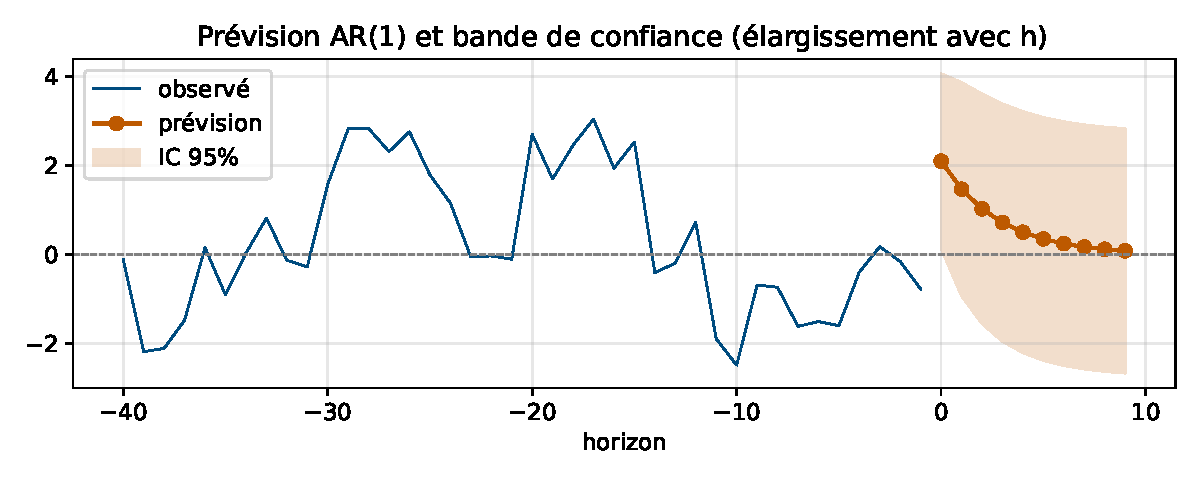
\includegraphics[width=0.86\textwidth]{forecast.pdf}
\caption{Prévision d'un AR(1) : la prévision converge vers la moyenne et la bande de
confiance s'\textbf{élargit} avec l'horizon (puis se stabilise).}
\end{figure}
\begin{lecture}[la bande de confiance]
L'incertitude $\sqrt{\sum_{j<h}\psi_j^2}$ \emph{croît} avec $h$ : on prévoit d'autant moins
précisément que l'horizon est lointain. Pour un AR(1) stationnaire la variance d'erreur tend
vers $\gamma(0)=\sigma^2/(1-\phi^2)$ ; pour un MA(1) elle est constante dès $h\ge2$.
\end{lecture}
\begin{recette}[Prévision $+$ IC, méthode ; $\to$ Q\,E.1--E.7, J.2]
\textbf{1.} Calculer $\widehat X_{n+h}$ (chocs futurs $=0$). \textbf{2.} Coefficients $\psi_j$.
\textbf{3.} $\Var(\Delta_h)=\sigma^2\sum_{j<h}\psi_j^2$. \textbf{4.}
IC $=\widehat X_{n+h}\pm1.96\,\sigma\sqrt{\sum_{j<h}\psi_j^2}$.
\end{recette}
\begin{exemple}[$\to$ Q\,E.1]
MA(1) $X_t=2+a_t+0.8a_{t-1}$, $\sigma^2=2$, $a_t=1.6$ : $\widehat X_{t+1}=2+0.8(1.6)=3.28$,
IC $=3.28\pm1.96\sqrt2$ ; $\widehat X_{t+2}=2$, IC $=2\pm1.96\sqrt{(1+0.64)2}=2\pm1.96\sqrt{3.28}$.
\end{exemple}

\vfill
\begin{center}\small\color{gris}
Cours réécrit pour la préparation au module --- d'après F.~BADAOUI (INSEA).
\end{center}
\end{document}
